\documentclass[runningheads,a4paper]{llncs}

\usepackage{amssymb}
\setcounter{tocdepth}{3}
\usepackage{graphicx}
\usepackage{subfig}
%\linespread{2}

\usepackage{url}
\usepackage{csquotes}
\newcommand{\keywords}[1]{\par\addvspace\baselineskip
\noindent\keywordname\enspace\ignorespaces#1}

\usepackage{listings}
\usepackage{color}
\usepackage{enumitem}
\usepackage{hyperref}

\definecolor{dkgreen}{rgb}{0,0.6,0}
\definecolor{gray}{rgb}{0.5,0.5,0.5}
\definecolor{mauve}{rgb}{0.58,0,0.82}

\lstset{frame=tb,
  language=C++,
  aboveskip=3mm,
  belowskip=3mm,
  showstringspaces=false,
  columns=flexible,
  basicstyle={\small\ttfamily},
  numbers=left,
  numberstyle=\tiny\color{gray},
  keywordstyle=\color{blue},
  morekeywords={vector},
  commentstyle=\color{dkgreen},
  stringstyle=\color{mauve},
  breaklines=true,
  breakatwhitespace=true,
  tabsize=3
}

\begin{document}

\mainmatter  % start of an individual contribution

% first the title is needed
\title{c3particles: \\ Modeling a Particle System in C++}

% a short form should be given in case it is too long for the running head
\titlerunning{c3particles}

%
\author{Rosalie Kletzander}
%
\authorrunning{c3particles}
% (feature abused for this document to repeat the title also on left hand pages)

\institute{Practical Course "Advanced Software Development with Modern C++"\\Summer Term 2018\\Institute for Computer Science\\
Ludwig-Maximilians-Universit\"at M\"unchen\\
}

\maketitle


%\begin{abstract}
%
%
%%keywords{network operating systems, programmable networks, Software-Defined Networking, SDN-controllers}
%\end{abstract}

\section{Introduction}
Particle systems are used in many different areas: most prominently in the entertainment industry in games and movies and for simulations and visualizations scientific research. No matter the area of application, the basic rules governing these systems are the same: the laws of physics. c3particles (cpp particles) implements a model of a particle system in C++ that separates the physical concepts and laws from the underlying graphics library. This enables a mathematical formulation of the forces influencing the particles.


\section{A Short Recap of Mechanical Physics}

In order to model a particle system that simulates natural phenomena, it is necessary to first understand the basic rules of motion.

Newton's First Law of Motion states:
\begin{quotation}
``Every object in a state of uniform motion tends to remain in that state of motion unless an external force is applied to it." \cite{Newton}
\end{quotation}

This means that an object will not move unless it is accelerated by a force, which brings us to Newton's Second Law of Motion:
\begin{quotation}
``The relationship between an object's mass \emph{m}, its acceleration \emph{a}, and the applied force \emph{F} is $ F = m*a $."  \cite{Newton}
\end{quotation}

With this information it is possible to calculate the acceleration of an object by dividing the applied force by the object's mass. The next step is deriving the velocity and location of the object per time step by integration \cite{strommer}.

The velocity of an object can be calculated by integrating the acceleration over time t. 
\begin{equation}
\overrightarrow{v}(t) = \int \mathrm{(\overrightarrow{a})} \mathrm{d}t = \overrightarrow{a}*t + C_v
\label{eq:vel}
\end{equation}

C is the integration constant, in this case it is equal to the velocity of t-1 for discrete time steps. Integrating the velocity over t yields the location.

\begin{equation}
\overrightarrow{s}(t) = \int \mathrm{(\overrightarrow{v})} \mathrm{d}t = \int (\overrightarrow{a}*t + C_v) \mathrm{d}t = \frac{\overrightarrow{a}*t^2}{2} + C_v + C_s
\label{eq:loc}
\end{equation}

Analogous to $C_v$, $C_s$ is equal to the location at t-1.

With these formulas, it is possible to calculate an object's change in location over time.

A further basic law of physical mechanics is the superposition principle, which states that applying the sum of two forces to an object has the same effect as if they were applied individually. Or, more formally:

\begin{equation}
f(a * x) = a * f(x)
\label{eq:superpos1}
\end{equation}
\begin{equation}
f(x + y) = f(x) + f(y)
\label{eq:superpos2}
\end{equation}

\cite{wiki}

These laws serve as the foundations of the physical model of the particle system. 

\section{Modeling the Particle System}
The basic concepts needed in order to model the particle system are already given by the physics described in the previous section. In fact, a particle system is a fairly simple construct. It contains objects, its "particles", which behave according to newtonian physics, i.e. "newtonian objects". They have a location, velocity, acceleration and mass. As Newton's First Law states, a force needs to be exerted in order for a particle to move. Since movement is merely a change of location over time, time also needs to be considered.

\subsection{Concepts}
In fact, these two concepts, "newtonian object" and "force" are sufficient for modeling a particle system. The basic .. expressions ..:

\paragraph{Particle $\ll$ Force}
applies a force to a particle using the formulas \ref{eq:vel} and \ref{eq:loc}

\paragraph{Force calc\_force(Particle, Particle, Function)}
calculates a force between two particles using the supplied function, when given the same particle twice, it returns the additive identity

\paragraph{Force gravity(Particle, Particle, List params)}
a specialization of calc\_force for calculating the gravitational force between two particles (is not actually a concept, but shows what calc\_force is capable of)

\paragraph{Force accumulate(Particle, ParticleContainer, Function)}
calc\_force for p with each other p in the container and reduce (addition) to one force

\paragraph{Force accumulate(Particle, ParticleContainer, List params, Function)}
use a pre-defined function to calculate the forces, pass initializer list for parameters

paragraph{Force accumulate(List forces)}
sum up a set of forces

\subsection{Time}
As the particle system is made to be rendered on a screen in (semi) real time, the frame per second count gives discrete time steps that are used for integrating over acceleration. For each frame, one time step is calculated, which simplifies the result of formula~\ref{eq:loc}:

\begin{equation}
\frac{\overrightarrow{a}*t^2}{2} + C_v + C_s = \frac{\overrightarrow{a}}{2} +C_v + C_s
\label{eq:simpleloc}
\end{equation}

%examples why it is cool: reverse, 

\section{Implementation}

c3particles contains several separate modules (Figure~\ref{fig:sysdia}. The Particle System module contains the physical model and uses input given by the user to select forces. It updates the particles that are then read by the Particle Renderer, which uses the location to calculate the vertices and faces that need to be drawn. It passes the vertex buffers of all the particles to the OpenGL Rendering Pipeline, which processes them accordingly. It then writes the framebuffer to the screen and triggers a new calculation.

%\begin{itemize}
%\item system diagram

%\item for each time step (signaled by OpenGL), the Particle System module calculates the new values for all the particles based on the input given by the user control window. These values are then read by the Particle Renderer and used to fill the vertex buffers depending on the visualization selected (e.g as points or cubes)
%\item then, the OpenGL Rendering Pipeline renders the frame, using the provided shaders
%\item as soon as the screenbuffer is swapped, the calculation for the next frame is started
%\end{itemize}

\textbf{
\begin{figure}[]
\centering
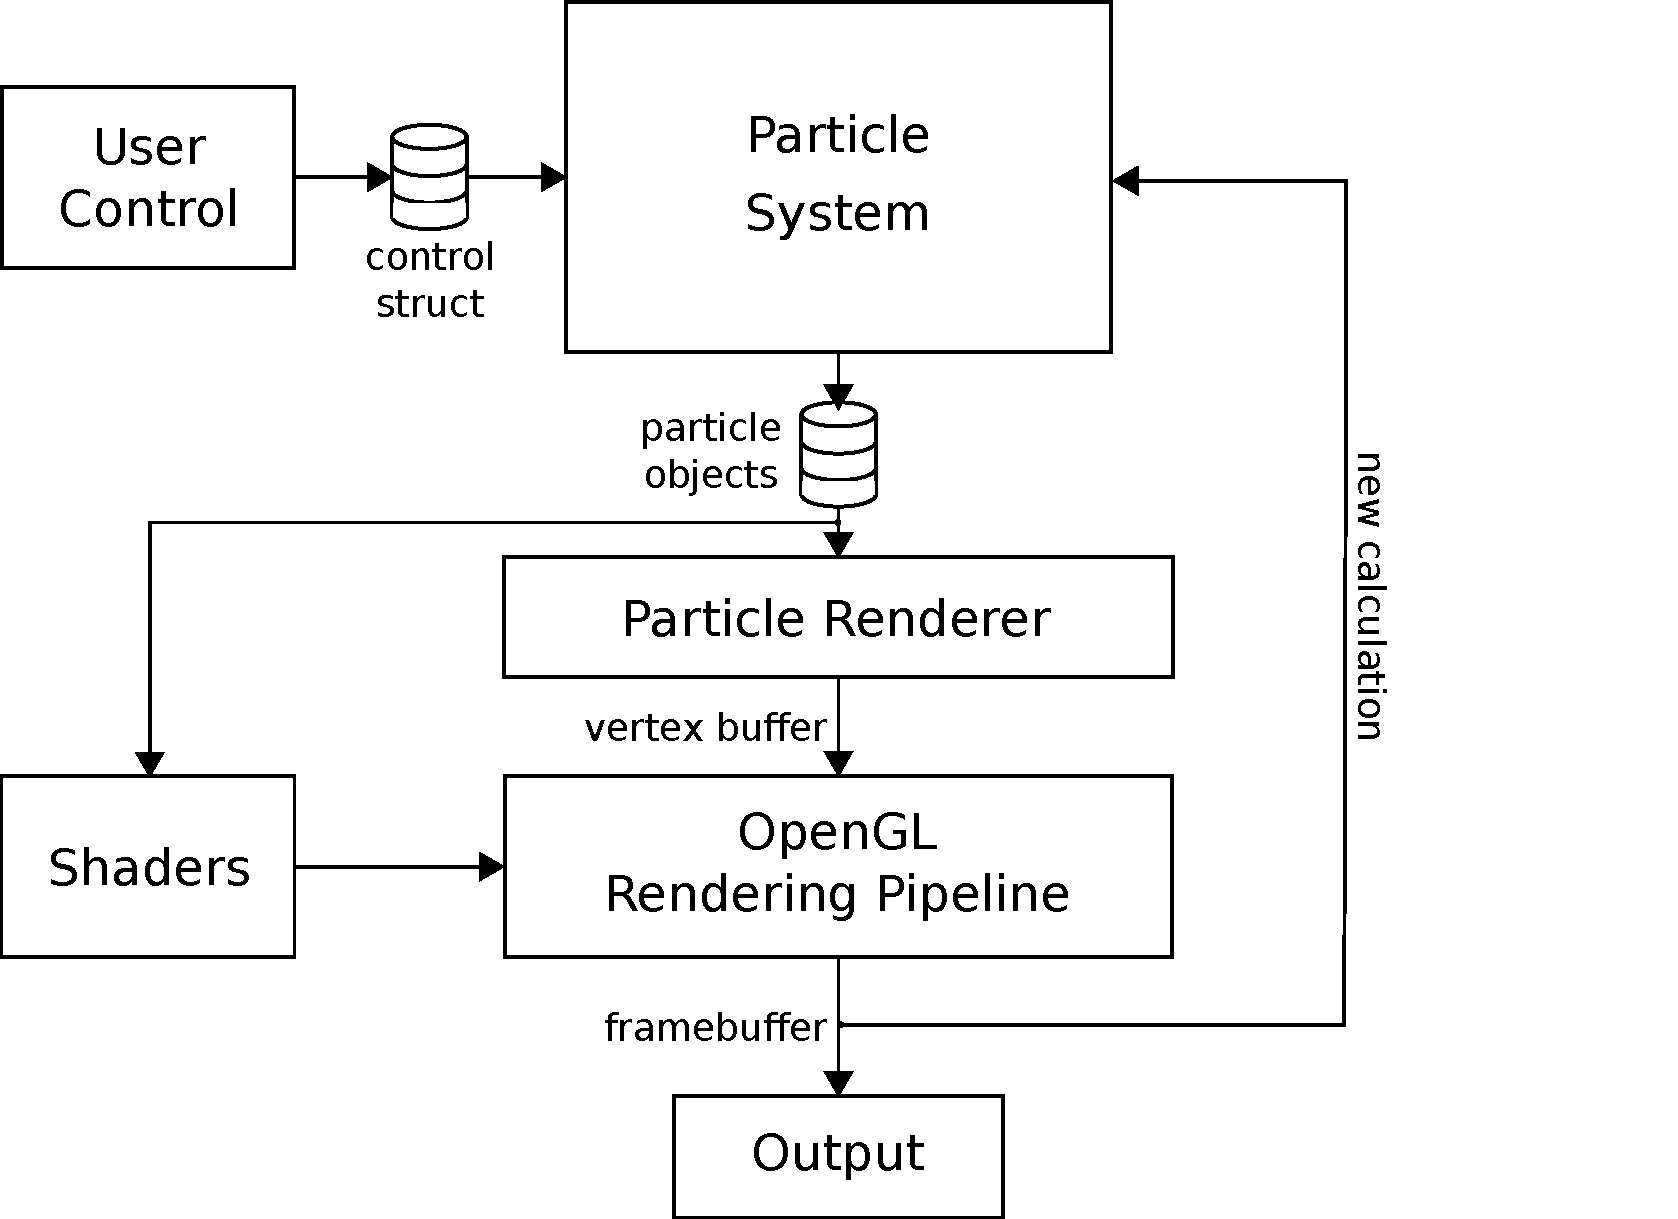
\includegraphics[width=0.8\textwidth]{images/system-diagram.pdf}
\caption{c3particles system diagram}
\label{fig:sysdia}
\end{figure}
}

\subsection{Particle System}
The Particle System module contains the physical model of the particle system and the particle objects (Figure~\ref{fig:sysdiadetail})
The physical model includes algorithms for calculating the forces on the particles, and the particles themselves. For each frame, the old values of the particles are read and used to update to the new values. The functions used to update the values are taken directly from formulas~\ref{eq:vel} and \ref{eq:simpleloc}.

\textbf{
\begin{figure}[]
\centering
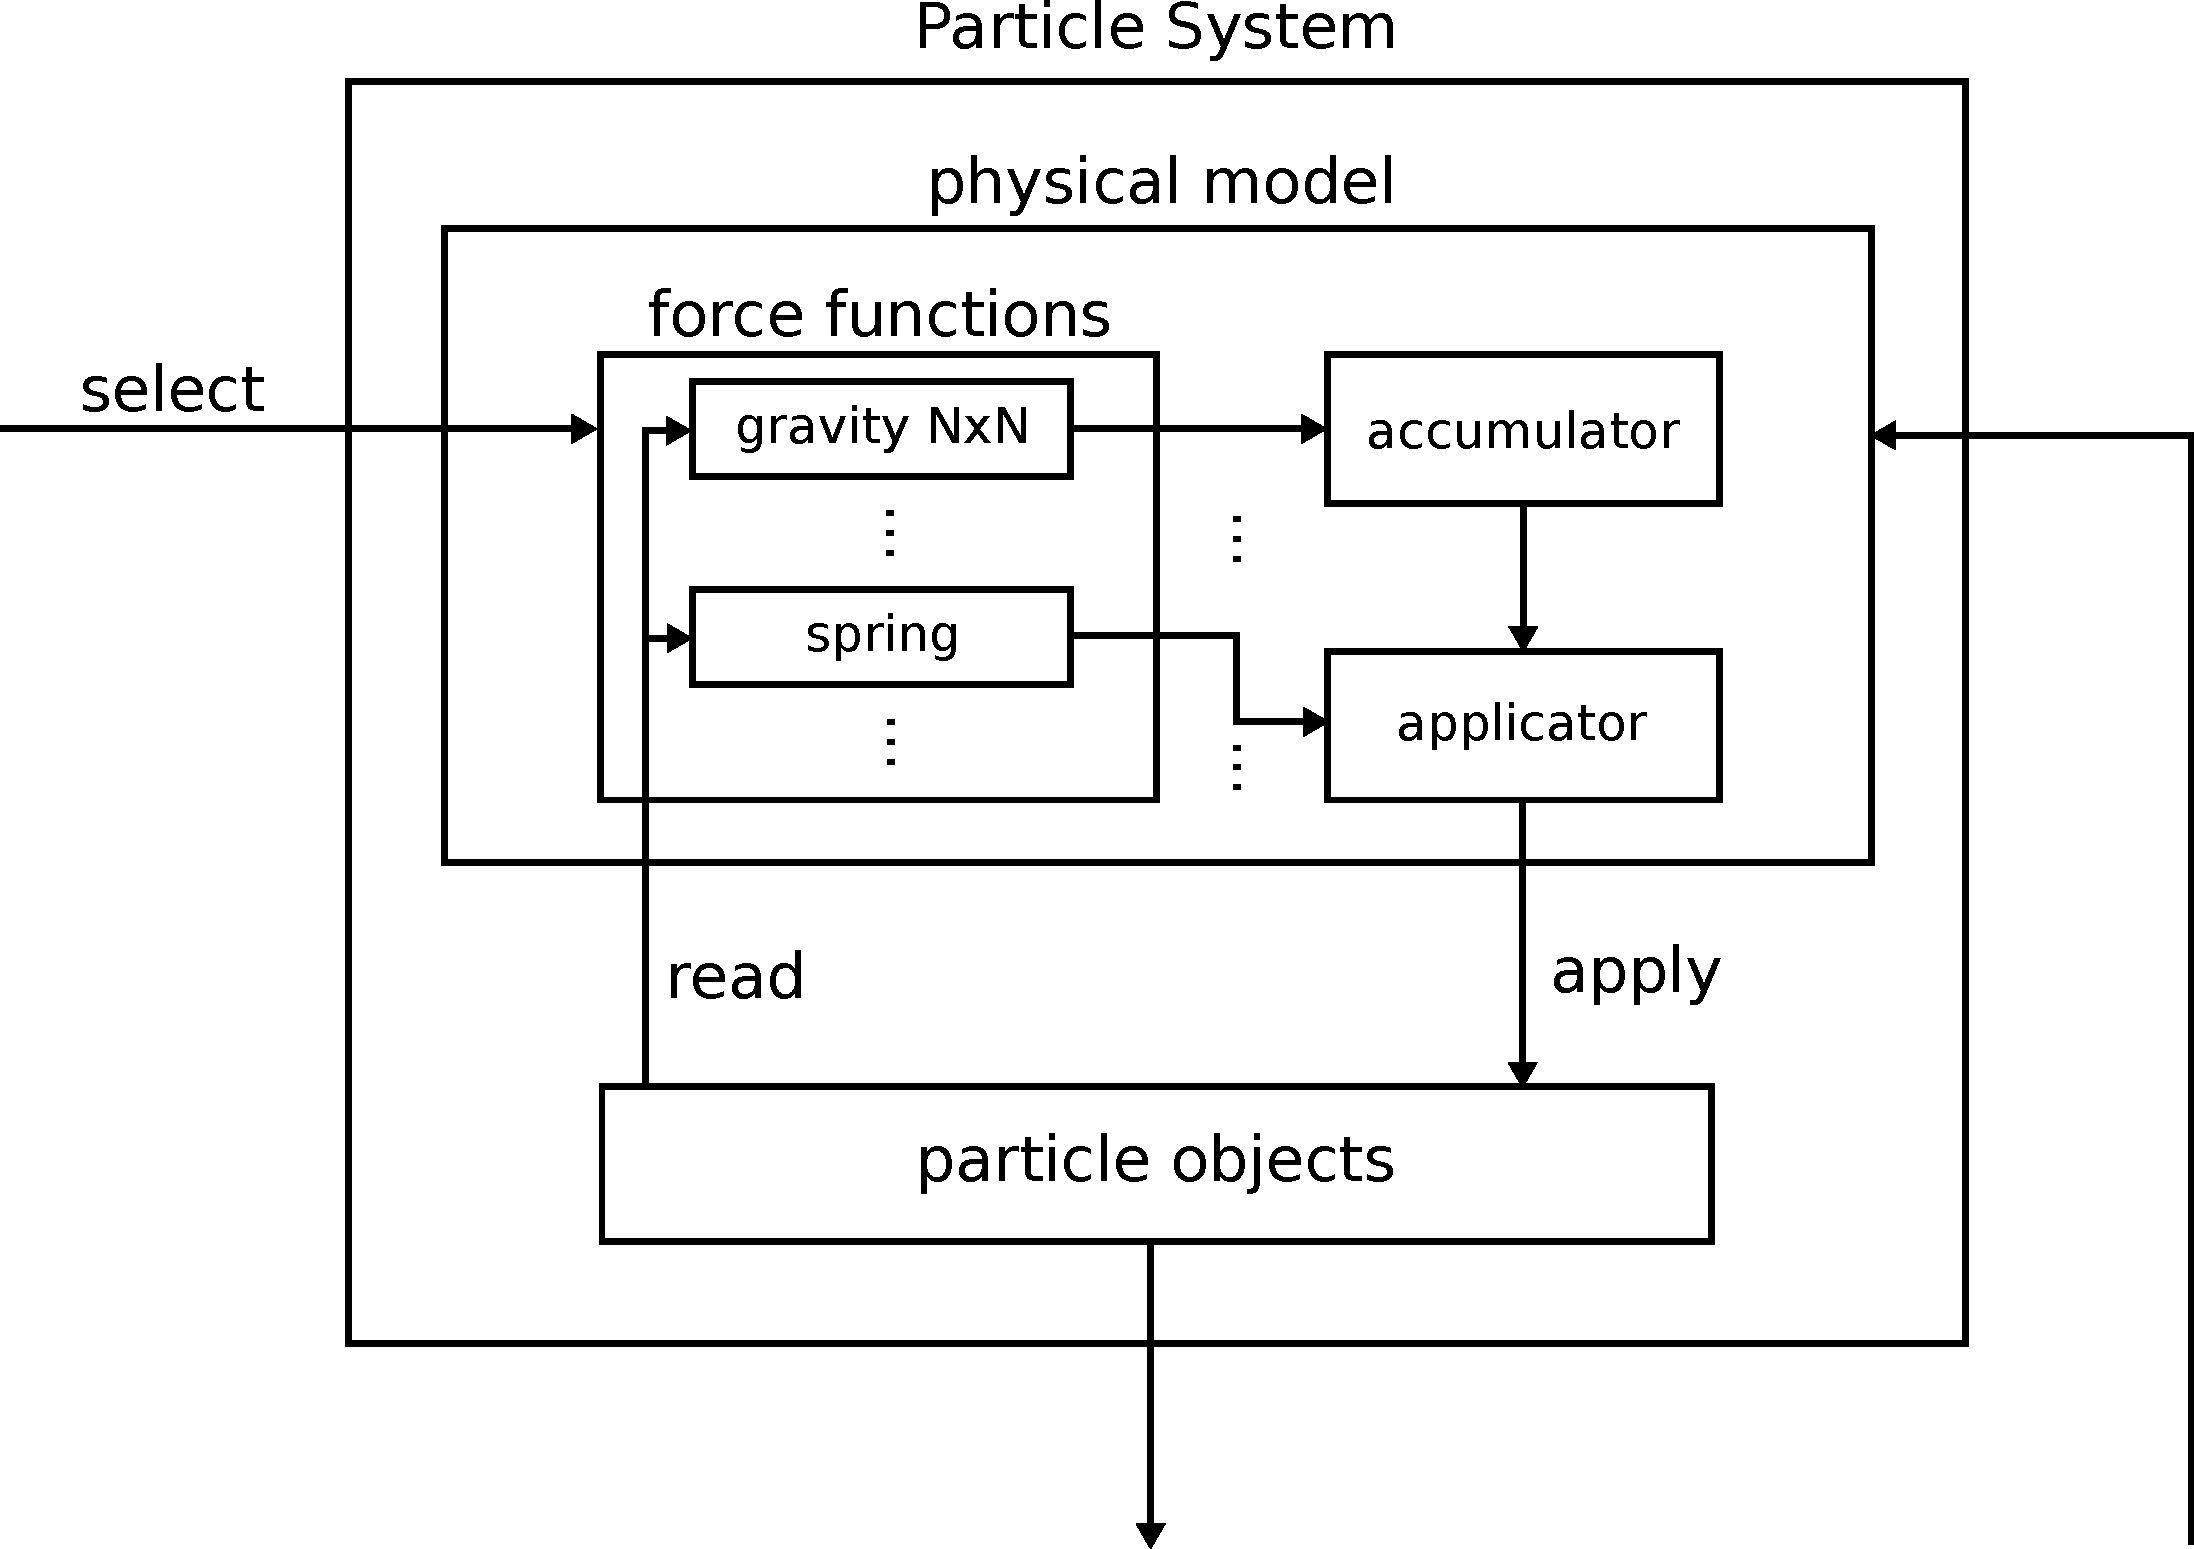
\includegraphics[width=0.8\textwidth]{images/particle-system-detail.pdf}
\caption{detailed diagram of the particle system}
\label{fig:sysdiadetail}
\end{figure}
}

\begin{figure}[tb]
\begin{lstlisting}
void ParticleSystem::update()                                                              
{                                                                                          
  // deltaT will always be 1.0 because calculation is based on frames                               
  for (Particle &p : _particles)                                                           
    {                                                                                      
      //v(t) = a*t + v(t-1)                                                            
      p.velocity = p.acceleration * 1.0f + p.velocity; //deltaT = 1.0                                  
                                                                                           
      //s(t) = (a*t^2)/2 + v(t) + s(t-1)                                               
      p.location = (p.acceleration * 1.0f) / 2.0f
      			   + p.velocity + p.location;
                                       	
      //acceleration is not accumulative, but recalculated at each time step          
      p.acceleration = {0, 0, 0};
    }                                                                                      
}                                                            
\end{lstlisting}
 \caption{ParticleSystem::update()}
 \label{fig:update}
\end{figure}

\subsubsection{Algorithms}
\begin{itemize}
\item concepts and expressions come to fruition here
\item differentiation between "external" forces and inter-particle forces
\item apply force $"<<"$
\item calc\_force
\item accumulate
\item specializations of calc\_force, e.g. gravity
\end{itemize}

The concepts and expressions defined above are incorporated into the system's algorithms. The core algorithm is calc\_force (Listing~\ref{fig:calcforce}), which takes a lamda defining the calculation of a force between two particles. 

\begin{figure}[tb]
\begin{lstlisting}
// calculates a force between two particles using the function ff
// when given the same particle twice, it returns the identity
Force calc_force(
    const Particle &p1,
    const Particle &p2,
    std::function<Force(const Particle &p1, const Particle &p2)> ff)
{
  if (&p1 == &p2)
    { return glm::vec3(0, 0, 0); }
  return ff(p1, p2);
}                                    
\end{lstlisting}
 \caption{calc\_force function}
 \label{fig:calcforce}
\end{figure}

This enables very straightforward definition of any force between two particles. It can be used to describe forces on the fly, or to create pre-defined force functions, such as gravitational force (Listing~\ref{fig:gravity}).

\begin{figure}[tb]
\begin{lstlisting}
// uses calc_force to calculate gravitational force between two particles
Force gravity(const Particle &p1,
			  const Particle &p2,
              std::initializer_list<float> params)
{
  Force result = calc_force(p1,
  							p2, 
  						    [p1, p2](const Particle &, const Particle &) {
        glm::vec3 direction = p2.location - p1.location;
        float gforce = (p1.mass * p2.mass) / pow(glm::length(direction), 2);
        glm::normalize(direction);

        return (gforce * direction);
      });
  // multiply by gravity constant
  for (auto c : params)
    {
      result *= c;
    }
  return result;
}               
\end{lstlisting}
 \caption{gravity function}
 \label{fig:gravity}
\end{figure}


For the calculation of the forces it is helpful to split them logically into "inter-particle forces" and "external forces". The former refers to the forces that exist between all pairs of particles (e.g. gravitational forces) and the latter refers to forces that are applied to each particle independently of all others (e.g. wind). 

\begin{figure}[tb]
\begin{lstlisting}
//iterate over all particles in the particle system
std::for_each(ps.begin(), ps.end(), [&ps](c3p::Particle& p)
{

  	//gravitational forces between particles
	p << c3p::accumulate(p,
						 ps.particles(),
						 {ps.g_constant()},
    					 c3p::gravity);
    					 
	// spring force from virtual particle at (0,0,0) to each particle
	p << spring(p, Particle(0,0,0), {spring_constant, spring_length);

	// simple user-defined attraction force pulling towards (0,0,0)
	p << calc_force(p, Particle(), [p](const Particle &, const Particle &)
	{
    	glm::vec3 direction = glm::normalize(glm::vec3(0,0,0) - p.location());
		return direction * 0.1;
    });
}          

//calculate new location from acceleration
ps.update();     
\end{lstlisting}
 \caption{example of how forces are applied}
 \label{fig:main}
\end{figure}

\emph{c3p::accumulate} (Listing~\ref{fig:main}, line 6) calculates the forces between each pair of particles (i.e. inter-particle forces) and reduces them. The result is a force that can then be applied normally.


\subsubsection{Particle Container}
The particles need to be stored in some data structure. At the moment, this is a std::vector which provides all the needed operations.

\subsection{User Control Window}
The user controls are implemented with GTK+\cite{gtk}. The control window runs in a different thread that fills a C struct with the values set by the user. These values are then read by the system in order to calculate the desired forces.

\subsection{Particle Renderer}
The particle renderer iterates over the particles in the particle system and fills the vertex buffers for each one. How the vertex buffers are filled depends on the function called. At the moment, it is possible to render the particles as pixels with no depth perception and uniform size (\emph{c3p::ParticleRenderer::renderPoints}
or as cubes (\emph{c3p::ParticleRenderer::renderCubes}). The size of the cubes depends on the size of the particle (which, at the moment is dependent on its mass). The vertex buffers are then passed to the OpenGL Rendering Pipeline.

\subsection{Shaders}

\subsection{Graphics Engine}
The graphics engine is only secondary for this project. OpenGL\cite{opengl} was chosen because of its prominence, however, with an appropriate particle renderer, any one could be used.

\section{Assets of c3particles}
\begin{itemize}
\item mathematical functions can be easily applied
\item clean separation allows for easy access to velocity etc (for reflection, reverse)
\end{itemize}

\section{Complexity and Possible Optimizations}
\begin{itemize}
\item complexity of naive implementation of inter-particle forces is $O(n^2)$
\item complexity of application of external forces and also updating is O(n)
\item force matrix for inter-particle forces
\item parallelize particle calculation (works very well, because applyforce only updates acceleration, so location and velocity are unchanged until all forces have been calculated)
\item well suited for offloading to the GPU
\item binary space partitioning for forces that are inversely proportional to distance
\item no pruning because particles that are outside of the viewport still exert forces 
\end{itemize}


\bibliography{literature}
\bibliographystyle{plain}

\end{document}
